% 66-31(66쪽) — 제2사분면의 점 $\pt{P}\left(-\dfrac{\sqrt{3}}{2},\,a\right)$ 와 동경 $\pt{OP}$(원문 「오른쪽 그림」). 스캔 화질이 낮아 TikZ 로 다시 그림.
% 라벨은 원문 것만: 점 이름과 좌표, $r$, $\theta$, $\pt{O}$, 두 축. $ar$ 의 값(답)이 읽히지 않게 눈금은 적지 않는다.
\begin{tikzpicture}[line width=0.6pt, >=stealth]
  \draw[->, line width=0.7pt] (-2.35,0) -- (1.45,0) node[below=1pt] {$x$};
  \draw[->, line width=0.7pt] (0,-0.95) -- (0,2.35) node[right=1pt] {$y$};
  \draw[line width=0.5pt] (0,0) -- (120:1.9);
  \draw[line width=0.4pt] (0.78,0) arc (0:120:0.78);
  \fill (120:1.9) circle (2.2pt);
  \node[font=\small] at (0.42,1.02) {$\theta$};
  \node[font=\small] at (-0.80,0.68) {$r$};
  \node[anchor=south east, font=\small] at (-0.86,1.72) {$\pt{P}\!\left(-\dfrac{\sqrt{3}}{2},\,a\right)$};
  \node[anchor=north east, font=\small] at (-0.04,-0.06) {$\pt{O}$};
\end{tikzpicture}
